%************************************************
% Grundlagen
%************************************************
\chapter{Grundlagen}
\label{sec:basics}

In diesem Kapitel werden einige Grundlagen vermittelt, auf welche in späteren Teilen dieser Arbeit verwiesen wird. Aus den Abschnitten "\nameref{sec:basics:playful-learning}" und "\nameref{sec:basics:mini-languages}" werden zudem Anforderungen an diese Arbeit abgeleitet.

%************************************************
% Spielerisches Lernen
%************************************************
\section{Spielerisches Lernen}
\label{sec:basics:playful-learning}

Die im Rahmen dieser Arbeit entwickelte Software soll Lehrer dabei unterstützen, ihren Schülern die Grundlagen des Programmierens zu vermitteln. Dies soll spielerisch geschehen. Prensky führt in seinem Buch \textit{Digital Game-Based Learning} drei Gründe an, warum digitales spielerisches Lernen funktioniert~\cite[147]{prensky2007}:

\begin{enumerate}
    \item Der erste Grund ist das zusätzliche Engagement, das dadurch entsteht, dass das Lernen in einen Spielkontext gebracht wird. Dies kann beträchtlich sein, besonders wenn Menschen nicht lernen wollen.
    \item Der zweite Grund ist der interaktive Lernprozess. Dieser kann und sollte abhängig von den Lernzielen viele verschiedene Formen annehmen.
    \item Der dritte Grund ist die Art und Weise, wie die zwei ersten Gründe im Gesamtpaket zusammengefügt werden. Es gibt viele Möglichkeiten, dies zu tun, und die beste Lösung ist sehr kontextabhängig.
\end{enumerate}

Des Weiteren hängt der Lernerfolg auch immer stark davon ab, wie Spiele vom Lehrer letztendlich eingesetzt werden, aber auch der Stil des Spieles spielt eine Rolle. Damit Spiele -- Lehrspiele im speziellen -- Spaß bringen, müssen sie einige Anforderungen erfüllen. Malone stellt in seinem Artikel \textit{What Makes Computer Games Fun?} eine Checkliste auf, die sich in drei Kategorien gliedert und unter anderem die folgenden Fragen enthält~\cite[49]{malone1981}:

\begin{itemize}
    \item \emph{Herausforderung}: Hat das Spiel ein Ziel? Hat das Spiel einen variablen Schwierigkeitsgrad? Verfügt die Aktivität über mehrere Ziele, z.~B. Zählen von Punkten oder schnelle Reaktionen? Enthält das Programm Zufall? Enthält das Programm versteckte Informationen, die selektiv aufgedeckt werden?
    \item \emph{Fantasie}: Enthält das Programm eine emotional ansprechende Fantasie? Hängt die Fantasie instinktiv mit der in der Aktivität erlernten Fähigkeit zusammen? Ist die Fantasie eine nützliche Metapher?
    \item \emph{Neugierde}: Gibt es audio- und visuelle Effekte, um die Neugier der Sinne zu stimulieren? Gibt es Elemente, die die kognitive Neugier wie Überraschungen oder konstruktives Feedback stimulieren?
\end{itemize}

Diese Anforderungen sollten bei der Aufstellung der Anforderungen für das im Rahmen dieser Arbeit entwickelte Programm berücksichtigt werden, auch wenn sich aufgrund der für diese Art von Lernspiel notwendigen, im nächsten Abschnitt beschriebenen Mechaniken, nicht alle aufgestellten Anforderungen erfüllen lassen werden.

%************************************************
% Minisprachen
%************************************************
\section{Minisprachen}
\label{sec:basics:mini-languages}

Minisprachen sind Programmiersprachen, die speziell auf die Anforderungen von Programmieranfängern zugeschnitten sind, indem sie einen reduzierten Sprachumfang bieten, der speziell auf die Lösung einer bestimmten Klasse von Problemstellungen zugeschnitten ist und dabei die Grundprinzipien des Programmierens hervorhebt bzw. deren Erlernen fördert.

Warum das Erlernen von Programmierfähigkeiten mithilfe von Minisprachen im Gegensatz zu den breit genutzten Universalsprachen (wie z.~B. Java oder C) sinnvoll ist, erklären Brusilovsky et al., indem sie drei Probleme von Universalsprachen für die Anwendung zum Lernen nennen, die Minisprachen zu beheben versuchen \cite[67]{brusilovsky1997}:

\begin{itemize}
    \item Universalsprachen sind zu groß und zu idiosynkratisch. Die konzeptionelle Basis der Sprache bildet zusammen mit den Hauptprinzipien der Programmierung eine große Menge an Material. Anstatt die Grundprinzipien hervorzuheben, rufen die Sprachen nebensächlich Begriffe auf, die die Feinheiten der jeweiligen Sprache und deren Umsetzung, nicht aber die Hauptprinzipien der Programmierung widerspiegeln.
    \item Universalsprachen fördern nicht das Verständnis ihrer grundlegenden Aktionen und Kontrollstrukturen. Die Sprachen sind nicht visuell und ihre Grundfunktionen werden hinter einer undurchsichtigen Barriere ausgeführt. Wenn der Prozess der Programmausführung verborgen ist, entwickelt der Student ein In\-put-Out\-put-ori\-en\-tiertes Verständnis. Auf diese Weise behindert das Fehlen von visuellem Feedback die Beherrschung der Sprachsemantik.
    \item Da sich Universalsprachen an der Zahlen- und Symbolverarbeitung orientieren, sind die ersten möglichen Aufgaben, die beim Unterrichten der Sprache umgesetzt werden können, weit von den Alltagserfahrungen der Schüler entfernt. Die Entwicklung von Anwendungen, die sowohl informativ als auch interessant sind, erfordert das Erlernen einer beträchtlichen Untermenge der Sprache und das Schreiben recht großer Programme.
\end{itemize}

Brusilovsky et al. heben in Ihrem Artikel \textit{Mini-languages: a way to learn programming principles} einige sich daraus ergebende Eigenschaften von Minisprachen als besonders wichtig hervor \cite[73-74]{brusilovsky1997}:

\begin{itemize}
    \item Sowohl Syntax, als auch Semantik der Sprache sollten \emph{einfach} sein.
    \item Die Operationen der Minisprache sollten \emph{sichtbar} sein. Die meisten Operationen, die der Akteur ausführt, sollten sichtbare Änderungen in der auf dem Bildschirm dargestellten Mikrowelt vornehmen.
    \item Die Minisprache sollte für die vorgesehene Kategorie von Studenten \emph{attraktiv} und aussagekräftig sein.
    \item Die Sprache sollte \emph{dialogorientiert} sein. Das bedeutet, dass die Sprache Befehl für Befehl in einem Navigationsmodus ausgeführt werden kann (Einzelbefehlsausführung) und als Ganzes in einem Programmiermodus (komplexe Programmausführung).
    \item Die Sprache sollte \emph{modular} sein. Sie sollte einen Mechanismus zum Erstellen abstrakter Anweisungen (Prozeduren) enthalten. Alle Verfahren sollten unabhängige Einheiten sein. Eine solche Prozedur kann als neuer Befehl des Akteurs betrachtet werden, der sowohl im Navigations- als auch im Programmiermodus verwendet werden kann.
\end{itemize}

Eine Mikrowelt ist dabei eine einfache Darstellung der von für die Minisprache benötigten Komponenten. In ihr findet keine realistische Simulation statt, sondern sie beschränkt sich auf einen leicht zu überblickenden Kern, der mit Brettspielen vergleichbaren Regeln folgt. Diese Regeln sind typischerweise mit der Minisprache abgestimmt.

Aus der Liste dieser Anforderungen ergeben sich direkte Anforderungen an die für diese Arbeit entwickelte Minisprache (siehe \ref{sec:requirements:program}). Sie sind auch -- soweit das beurteilt werden kann -- in allen im nächsten Kapitel genannten vergleichbaren Arbeiten berücksichtigt.

In BlattWerkzeug wird die zu entwickelnde Minisprache mithilfe einer Grammatik definiert, die sich aus diesen Grammatiken ergebenden Syntaxbäume werden im nächsten Abschnitt vorgestellt.

%************************************************
% Syntaxbäume
%************************************************
\section{Syntaxbäume}
\label{sec:basics:syntaxtrees}

Der Syntaxbaum repräsentiert die Struktur eines Quelltextes, der mit dem Drag \& Drop-Edi\-tor in BlattWerkzeug (siehe \ref{sec:requirements:existing:structure:drag-drop}) bearbeitet wird. In einer konventionellen Entwicklungsumgebung würde man an dieser Stelle von einer Datei sprechen. Der Syntaxbaum als solcher ist nichts weiter als eine Datenstruktur, auf welcher Operationen zur Veränderung (einfügen, löschen, tauschen, \dots) definiert sind. Der Baum verfügt explizit über keinerlei Funktionalität zur eigenen Validierung oder zur Erzeugung von Programmcode. Er fungiert stattdessen als Eingabe für andere Module, welche diese Funktionalität bereitstellen~\cite[3]{riemer2018}.

Jeder Knoten eines Baumes entspricht mindestens einem Typen, welcher sich aus den Zeichenketten \inlinec{language} (im Sinne einer Programmiersprache) und \inlinec{name} zusammensetzt. Anhand dieses Typs entscheiden alle anderen Module, wie genau mit dem Knoten zu verfahren ist~\cite[4]{riemer2018}.

Die Speicherung von atomaren Daten erfolgt im Syntaxbaum durch die Verwendung sogenannter Eigenschaften (engl. Properties). Dabei handelt es sich um Zeichenketten, Zahlen oder Wahrheitswerte, welche über einen Schlüssel zugreifbar sind~\cite[4]{riemer2018}. In Abbildung \ref{fig:basics:syntaxtrees:1} ist ein Knoten \inlinec{const} einer Sprache \inlinec{math} dargestellt, welcher einen Integerwert repräsentiert. Dabei ist der eigentliche Wert in der Eigenschaft \inlinec{value} definiert.

\begin{figure}[h]
  \centering
  \includegraphics[width=0.25\textwidth]{gfx/basics-syntaxtrees-1.graphviz.pdf}
  \caption{Beispielhafte Darstellung einer Konstante \inlinec|42|}
  \label{fig:basics:syntaxtrees:1}
\end{figure}

Kinder von Knoten werden in benannten Kindgruppen organisiert. Dabei handelt es sich um eine Verallgemeinerung der von XML bekannten Aufteilung in At\-tri\-but-Kin\-der und Ele\-ment-Kin\-der. Mit diesen Syntaxbäumen lassen sich die Kinder folglich beliebig in Unterbäumen organisieren~\cite[4]{riemer2018}. So ist in Abbildung \ref{fig:basics:syntaxtrees:2} ein Knoten \inlinec{operation} dargestellt, der jeweils eine Konstante für die linke und die rechte Seite als Kindknoten führt. Außerdem enhält der Knoten die Eigenschaft \inlinec{operation}, durch welche eine mathematische Operation festgelegt wird. Dieser Knoten kann so als eine Darstellung für den Ausdruck \inlinec{(41 + 1)} verstanden werden.

\begin{figure}[h]
  \centering
  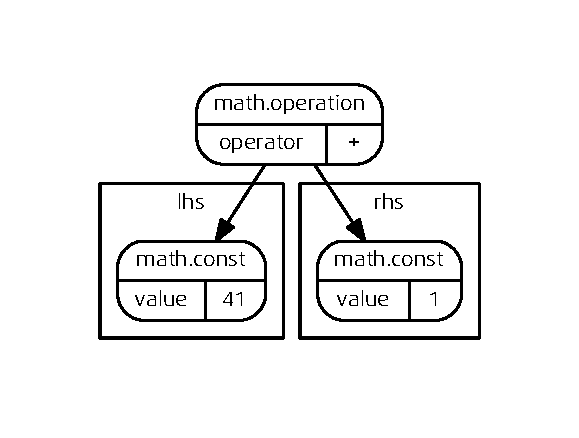
\includegraphics[width=0.45\textwidth]{gfx/basics-syntaxtrees-2.graphviz.pdf}
  \caption{Beispielhafte Darstellung einer Operation als Syntaxbaum}
  \label{fig:basics:syntaxtrees:2}
\end{figure}

Durch die Kindknoten ist eine Verschachtelung möglich. So ließe sich der Ausdruck \inlinec{(2 + (4 * 10))} durch den in Abbildung \ref{fig:basics:syntaxtrees:3} dargestellten Syntaxbaum repräsentieren.

\begin{figure}[h]
  \centering
  \includegraphics[width=0.55\textwidth]{gfx/basics-syntaxtrees-3.graphviz.pdf}
  \caption{Beispielhafte Darstellung einer verschachtelten Operation als Syntaxbaum}
  \label{fig:basics:syntaxtrees:3}
\end{figure}

Die gezeigten Graphen dienen an dieser Stelle der Übersicht. Intern werden Syntaxbäume in BlattWerkzeug als JSON-Do\-ku\-mente verwaltet.

Die Verwendung und Benennung von Eigenschaften und Kindknoten ist nicht beliebig. Sie wird durch eine Grammatik definiert, welche im nächsten Abschnitt beschrieben ist.

%************************************************
% Grammatiken
%************************************************
\section{Grammatiken}
\label{sec:basics:grammars}

Die Grammatik definiert die grundsätzlich zulässigen Strukturen eines abstrakten Syntaxbaumes. Aus dieser Beschreibung lassen sich unmittelbar Validatoren zur Überprüfung von Syntaxbäumen erzeugen. Nimmt man zu dieser Beschreibung noch spezielle Ge\-ne\-ra\-tor-An\-wei\-sung\-en dazu, können aus einer Grammatik auch Blocksprachen erzeugt werden~\cite[3]{riemer2018}.

Das folgende Beispiel leitet eine Grammatik her, welche sich zum Validieren von einfachen mathematischen Ausdrücken eignen würde. Die damit validierbaren Syntaxbäume sind bereits aus dem vorherigen Abschnitt \ref{sec:basics:syntaxtrees} bekannt. Abbildung \ref{fig:basics:grammars:1} zeigt dafür eine Grammatik, welche lediglich Bäume aus einer Konstanten mit einem Wert als valide auffassen würde (in Anlehnung an~\cite[6]{riemer2018}).

\begin{figure}[h]
  \lstinputlisting{snippets/baics-grammars-grammar-1.txt}
  \caption{Grammatik mit Knoten für Konstante}
  \label{fig:basics:grammars:1}
\end{figure}

Die Definition eines erlaubten Knotens wird mit node eingeleitet, der im Syntaxbaum zu verwendende Typname ergibt sich aus dem Namen der Grammatik (\inlinec{math}) und dem Namen des Knotens (\inlinec{const}). In diesem konkreten Fall darf ein valider Knoten lediglich über eine einzige Eigenschaft (\inlinec{prop}) \inlinec{value} verfügen, nicht jedoch über Kindknoten. Die mit \inlinec{prop} definierte Eigenschaft ist auf Integerwerte beschränkt. Ein im Sinne dieser Grammatik valider Baum hätte also einen einzigen Knoten vom Typ \inlinec{math.const} mit einer Eigenschaft \inlinec{value} (in Anlehnung an~\cite[6]{riemer2018}).

\begin{figure}[h]
  \lstinputlisting{snippets/baics-grammars-grammar-2.txt}
  \caption{Grammatik mit Knoten für Konstanten und Operationen}
  \label{fig:basics:grammars:2}
\end{figure}

Desweiteren ist es möglich, Beziehungen zwischen Knoten zu definieren. Die Anweisung \inlinec{children} innerhalb einer \inlinec{node}-De\-fi\-ni\-ti\-on erwartet zunächst die Angabe eines Namens und dann folgt mit \inlinec{::=} getrennt eine an Produktionsregeln angelehnte Aufzählung der zulässigen Typen in dieser Kindgruppe~\cite[6]{riemer2018}.

Innerhalb dieser "Produktionsregeln" können die Typen mit den bekannten Quantifizierern \inlinec{*} (beliebig häufig), \inlinec{+} (mindestens ein Mal) und \inlinec{?} (optional) versehen werden. Exakte Häufigkeitsangaben sind ebenfalls möglich, die Syntax lehnt sich dabei an die erweiterte Backus-Naur-Form an~\cite[6]{riemer2018}.

Im konkreten Beispiel in Abbildung \ref{fig:basics:grammars:2} kann die Operation \inlinec{operation} sowohl auf ihrer linken, als auch auf ihrer rechten Seite genau eine Konstante aufnehmen. Außerdem ist die Eigenschaft des Operators auf eine der vier Grundrechenarten beschränkt.

Schließlich ist es mithilfe eines \inlinec{typedef} möglich, eine Menge von Knotentypen als Kindknoten zuzulassen. Im konkreten Beispiel in Abbildung \ref{fig:basics:grammars:3} ist es für den \inlinec{operation}-Kno\-ten möglich, eine Konstante oder sich selbst als Kindknoten aufzunehmen. Ein Ausdruck in der Form \inlinec{(1 + (2 * 3))} kann so realisiert werden.

\begin{figure}[h]
  \lstinputlisting{snippets/baics-grammars-grammar-3.txt}
  \caption{Grammatik mit \inlinec|typedef|}
  \label{fig:basics:grammars:3}
\end{figure}

Als Wurzelknoten für einen vollständigen Syntaxbaum ist immer nur der erstgenannte Knoten (oder auch \inlinec{typedef}) zulässig.

Eine Grammatikdefinition in dieser Form muss für die im Rahmen dieser Arbeit konzipierte Minisprache entwickelt werden.
